\documentclass{beamer}

\usepackage{fontspec}
\usepackage[ngerman]{babel}
\usepackage{csquotes}

% import the bib.bib bibliogrpahy
\usepackage{biblatex}
\addbibresource{bib.bib}

\usetheme{Berlin}
\usecolortheme{beaver}

\usefonttheme{professionalfonts} % using non standard fonts for beamer
\usefonttheme{serif} % default family is serif
\setmainfont{Liberation Serif}


\title{Einf\"uhrung in \LaTeX}
\author{Daniel Renschler}
\date{17. Juli 2023}


\begin{document}





\begin{frame}
    \titlepage 
\end{frame}




\begin{frame}
    \tableofcontents
\end{frame}



\section{\LaTeX?}
\begin{frame}{Was ist \LaTeX?}
    \begin{itemize}
        \item Erfinder
        \item warum er es erfand
    \end{itemize}

    \begin{columns}
        \column{0.7\textwidth}
        
        \column{0.3\textwidth}
        \begin{figure}[htpb]
            \centering
            \includegraphics[width=1\textwidth]{./l}
            \caption{}
        \end{figure}
    \end{columns}

\end{frame}



\begin{frame}{Warum \LaTeX?}
    \begin{itemize}
        \item Einfacher
        \item Logisch
        \item Bibliografie
        \item macht spa\ss
    \end{itemize}

\end{frame}



\begin{frame}{Nutzzwecke}

    \begin{itemize}
        \item Ausarbeitungen/Laborberichte
        \item Pr\"asentationen
        \item Dokumente
        \item B\"ucher
    \end{itemize}
\end{frame}




\begin{frame}{Berichte}
    \begin{itemize}
        \item Laborberichte 
    \end{itemize}
    \begin{figure}[htpb]
        \centering
        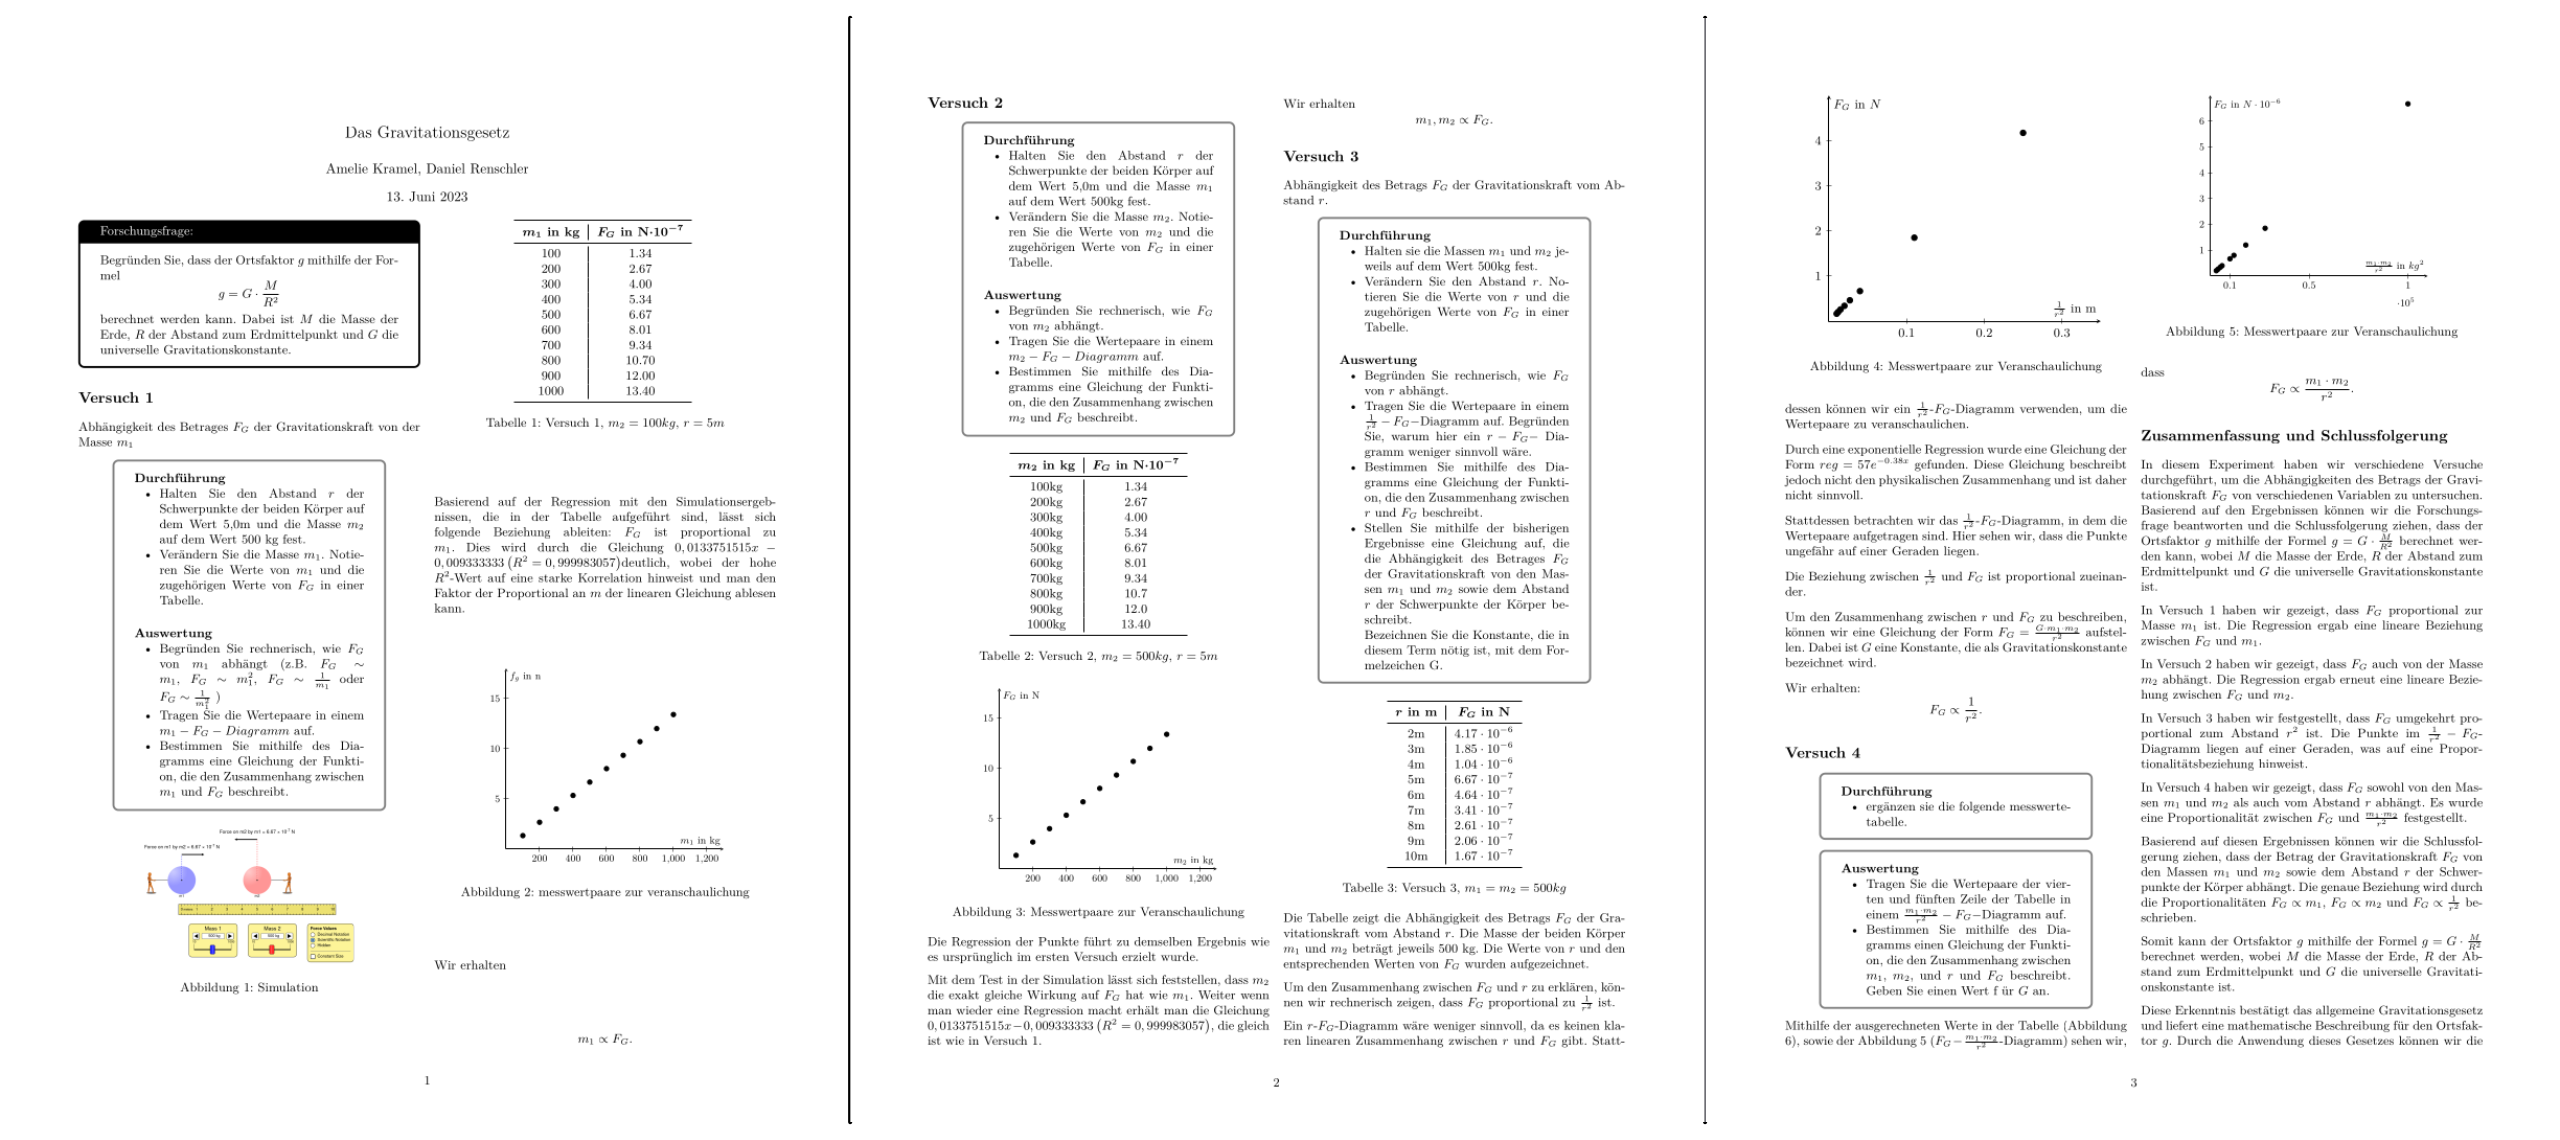
\includegraphics[width=1\textwidth]{./figs/am stueck.png}
        \caption{Laborprotokoll Gravitationsgesetz}
        \label{fig:}
    \end{figure}
\end{frame}



\begin{frame}{Paper}
    \begin{figure}[htpb]
        \centering
        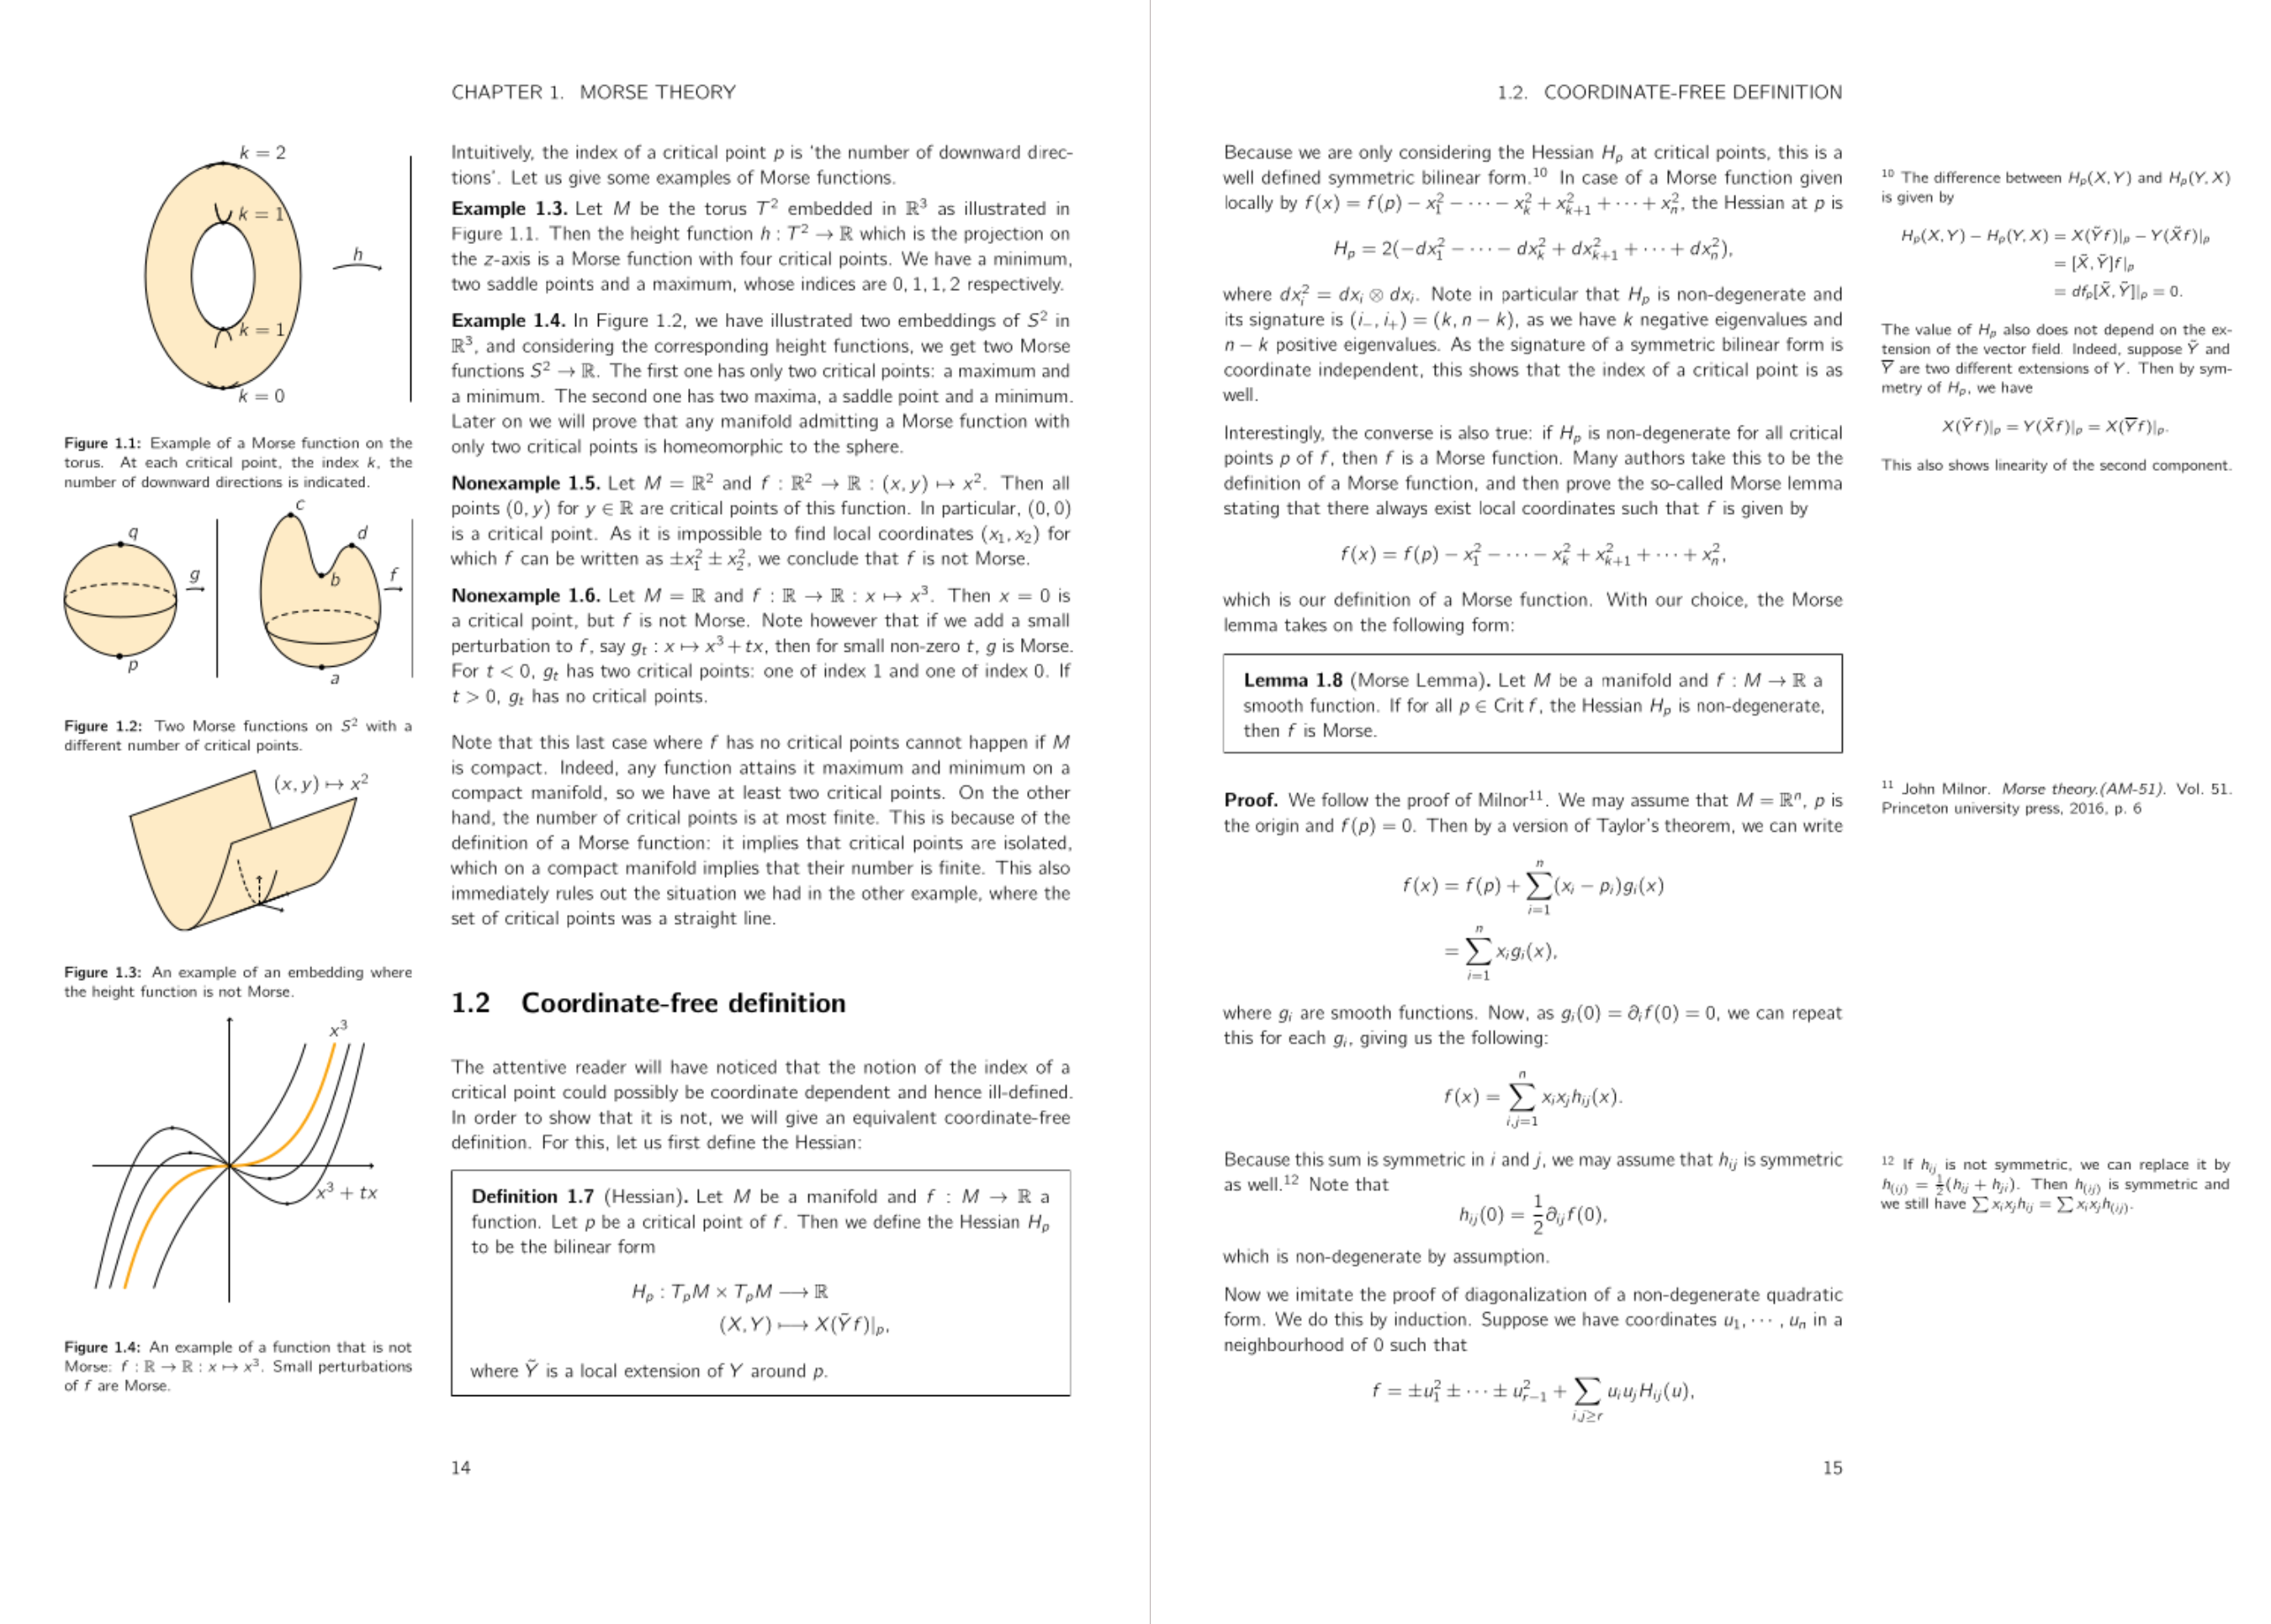
\includegraphics[width=0.7\textwidth]{./figs/example-paper.png}
        \caption{Auszug einer Masterarbeit \"uber Morse Theory}
    \end{figure}
\end{frame}



\section{Grundlegender Syntax}
\begin{frame}{Beispiel 1}


Beispiele:
\begin{itemize}
    \item Irgendwas mit Euler \cite{baranek2023randomized}
        \[ \mathcal{L} = \frac{\partial}{\partial t}+ \frac{1}{2}\sum_{k=1}^{m}\frac{\partial^2}{\partial y_{k}^2} .\] 
\end{itemize}


\begin{itemize}
    \item Analysis Aufgabe: 
        \[ \lim_{x\to \int_0^{\infty} \sqrt{t}e^{-t}dt}\left( \left( \sum_{n=0}^{\infty}\frac{x^{4n_4}}{(2n+1)(4n+3)(4n+4)} \right)''  \right) .\] 
\end{itemize}
\end{frame}

    



\begin{frame}
    Toeplitz Matrix
    \[ A=\begin{bmatrix}
            a_0 & a_{-1} & a_{-2} & \ldots & \ldots  &a_{-n+1}  \\
            a_1 & a_0  & a_{-1} &  \ddots   &  &  \vdots \\
            a_2 & a_1 & \ddots  & \ddots & \ddots& \vdots \\ 
            \vdots &  \ddots & \ddots &   \ddots  & a_{-1} & a_{-2}\\
            \vdots &         & \ddots & a_1 & a_0 &  a_{-1} \\
            a_{n-1} &  \ldots & \ldots & a_2 & a_1 & a_0
        \end{bmatrix} .\] 
\end{frame}



\begin{frame}{Physik Beispiel}
    Sequential Quantum Circuits as Maps between Gapped Phases.\cite{chen2023sequential}
    \begin{align*}
        \frac{1}{|G|}\sum_g X^g_i &\to \sum_h T^h_{i-1}T^h_i, \quad i=2,\ldots,N,  \\
        \frac{1}{|G|} \sum_g X_1^g &\to \frac{1}{|G|} \sum_{h,h'}e^{-\frac{2\pi i}{|G|}(h'-h)g}T_1^hT^{h'}_N \prod^N_{i=1}X_i^g,  \\
        \sum_h T^h_i T^h_{i+1} &\to \frac{1}{|G|} \sum_g X_i^g, i=2,\ldots,N  \\
        \sum_h T^h_1 T^h_2 &\to \frac{1}{|G|} \sum_g X_1^g \prod_{i=1}^N X_i^g.
    \end{align*}
\end{frame}












\begin{frame}{Literatur}
    \printbibliography
    
\end{frame}




%\begin{frame}{Text and Image in beamer}
%    \frametitle{test frametitle}
%    \section{test section}
%    \begin{columns}
%        \column{0.4\textwidth}
%        This is an example of text and image in the same slide using columns environment.
%        \hfill
%        \column{0.4\textwidth}
%        Lorem ipsum dolor sit amet, consectetur adipiscing elit, sed do eiusmod tempor incididunt ut labore et dolore magna aliqua. Ut enim ad minim veniam, quis nostrud exercitation ullamco laboris nisi ut aliquip ex ea commodo consequat. Duis aute irure dolor in reprehenderit in voluptate velit esse cillum dolore eu fugiat nulla pariatur.
%    \end{columns}
%\end{frame}



\end{document}
